\documentclass[twocolumn, 10pt]{article}
\usepackage[utf8]{inputenc}
\usepackage{booktabs}
\usepackage{geometry}
\usepackage{parskip}

% --- figures ---------------------------------------------------------------
\usepackage{graphicx}
\usepackage{dblfloatfix}          % allows figure* at the bottom of a page too
\usepackage[font=small,labelfont=bf]{caption}
\graphicspath{{figures/}}

% Reduced margins and set a standard column gap to maximize page space
\geometry{a4paper, margin=0.75in, columnsep=0.3in}

% Tighter paragraph spacing to prevent short paragraphs from wasting vertical space
\setlength{\parskip}{0.4em}

\title{Comparative Study of Hindi and Nepali Language Models}
\author{}
\date{}

\begin{document}

\maketitle

\begin{abstract}
In this project, I built two small language models, one for Hindi and one for Nepali. The main aim of the project was to study how the training data can affect the behaviour and performance of a language model. I wanted to keep the models as similar as possible so that the differences in the results can mainly be studied through the data.

I collected and cleaned separate datasets for both languages and trained separate tokenizers. Both tokenizers had a vocabulary size of 8,000. After this, I built two decoder only Transformer models from scratch using PyTorch. Both models had exactly the same architecture and had 25,379,840 parameters. The only major difference was the data used for training.

In the second phase, I evaluated the models using language modelling metrics, text generation and attention analysis. I found that different metrics gave different results. Hindi had better perplexity, while Nepali had better bits per character. This showed me that comparing two languages using only one metric can sometimes be misleading.

In the third phase, I finetuned both models on a synthetic reasoning dataset. The models were able to learn the required answer format, but they had a lot of difficulty with unseen entity names. This suggested that the models were learning some patterns and memorising names instead of actually solving the reasoning problem. I also found that aggressive finetuning caused a very large amount of forgetting. A smaller learning rate and only one epoch gave better results while keeping much more of the original language modelling ability.
\end{abstract}

\section{Introduction}
Large language models need a large amount of text for training. However, the amount and quality of available text is not the same for every language. This is especially important for languages which have less digital data available.

For this project, I selected Hindi and Nepali. Hindi can be considered the higher resource language and Nepali the lower resource language. Both languages use the Devanagari script, but they are still different languages and have different characteristics.

My main idea was to build two models which are exactly the same in terms of architecture. This was important because if I used different model sizes, it would become difficult to understand whether a difference came from the language data or from the model itself. Both models ended up having exactly 25,379,840 parameters, the same number of layers, same number of attention heads, same model size and same context length. The vocabulary was also 8,000 for both models.

I divided the project into three phases. In Phase 1, I collected the data, cleaned it, removed duplicates and trained the tokenizers. In Phase 2, I implemented and pretrained the Transformer models. In Phase 3, I finetuned the models on reasoning tasks and analysed how their behaviour changed.

The most important thing I learned from this project is that getting a good score is not always enough. I need to understand what the metric is actually measuring and whether the experiment was designed properly.

\section{Phase 1: Data Collection and Tokenizer}

\subsection{Data Collection}
I created separate data pipelines for Hindi and Nepali. I used both manually collected data and automatically collected data. The manual data included Wikimedia dumps and text collected from news, government and literary websites. The automated data mainly came from the AI4Bharat Sangraha dataset.

The project required at least 20 percent of the data to be manually collected. I achieved a manual share of 26.87 percent for Hindi and 21.20 percent for Nepali.

The final Hindi corpus had 520,409,408 tokens and the Nepali corpus had 632,711,308 tokens. There were 848,815 Hindi documents and 1,367,965 Nepali documents. The datasets were split at the document level into training, validation and test sets.

One of the most useful things I found during data cleaning was about duplicate documents. At first, it might seem that checking URLs is enough to remove duplicate articles. But I found that two Nepali crawl shards had 1,718 identical article texts while having zero URLs in common.

This means that the same article could appear on different websites or under different URLs. If I had only checked the URLs, all these duplicates would have remained in the dataset.

Because of this, I used SHA 256 hashes of the actual content for deduplication. This allowed me to identify documents which had exactly the same text even when their URLs were different.

I also found another problem when I audited the manual dataset. Only 42.7 percent of the original Nepali manual partition was unique. The problem happened because different collection runs were using different versions of the deduplication registry. Because of this, some runs could not see documents which were added by another run.

I found this problem during the audit and collected more data to fix it. This was an important lesson for me because it showed that a data pipeline can run without errors and still produce a bad dataset. Checking the final data is also very important.

\subsection{Vocabulary Size}
I selected a vocabulary size of 8,000 for both languages.

The main reason was the parameter budget. A vocabulary is not free in a language model because the token embedding matrix contains one vector for every token. With a model size of 512, every additional 1,000 vocabulary entries require another 512,000 parameters.

I compared different vocabulary sizes. Going from 4,000 to 8,000 gave a fertility improvement of 0.2638 while using about 1.02 million more parameters. Going from 8,000 to 16,000 gave an improvement of 0.1710 but required about 2.05 million additional parameters. From 16,000 to 32,000 the improvement was only 0.1048 while requiring about 4.10 million additional parameters.

So the improvement becomes smaller when the vocabulary becomes larger. A vocabulary of 32,000 would also use a very large part of the total parameter budget. Because of this, I decided that 8,000 was a reasonable choice.

Both tokenizers had an unknown token rate of 0 percent. I used byte fallback, so text which was not directly represented in the vocabulary could still be represented using UTF 8 bytes.

\subsection{BPE and Unigram}
I also compared BPE and Unigram tokenizers. Unigram gave slightly better fertility results, especially for Hindi. However, I selected BPE for the final models.

This was one decision where I did not completely follow the main criterion given in the project. The unknown token rate was 0 percent for all the tokenizers, so fertility would have selected Unigram.

I had other reasons for using BPE, such as keeping the tokenizer algorithm the same for both models and making the results easier to compare with existing Devanagari work.

However, I think this decision could have been stronger. I did not pretrain the same model using both tokenizers and compare their final validation loss. That would have been a better experiment to decide between them.

\subsection{Phase 1 Results}
The final statistics were as follows.

\begin{table}[h]
\centering
\begin{tabular}{lrr}
\toprule
Measure & Hindi & Nepali \\
\midrule
Corpus tokens & 520,409,408 & 632,711,308 \\
Documents & 848,815 & 1,367,965 \\
Manual share & 26.87\% & 21.20\% \\
Vocabulary & 8,000 & 8,000 \\
Fertility & 1.4938 & 1.5566 \\
Characters per token & 3.484 & 4.127 \\
Unknown token rate & 0.00\% & 0.00\% \\
\bottomrule
\end{tabular}
\end{table}

The Nepali corpus had more tokens than the Hindi corpus in the final dataset. However, calling Nepali a lower resource language refers to its general availability of digital data, not simply the number of tokens in my final corpus.

\section{Phase 2: Transformer Model and Pretraining}

\subsection{Model Architecture}
I implemented a decoder only Transformer from scratch using basic PyTorch layers. I did not use the ready made Transformer module.

Both models had exactly the same architecture.

\begin{table}[h]
\centering
\begin{tabular}{lr}
\toprule
Component & Value \\
\midrule
Parameters & 25,379,840 \\
Model size & 512 \\
Layers & 8 \\
Attention heads & 8 \\
Feed forward size & 1536 \\
Context length & 512 \\
Vocabulary size & 8,000 \\
Dropout & 0.1 \\
\bottomrule
\end{tabular}
\end{table}

I used weight tying between the token embedding and the final language modelling layer. This means that the same matrix is used for both operations. It saved around 4 million parameters.

I used a feed forward size of 1536 instead of 2048. Using 2048 would have made the model larger than the target parameter budget.

I also used pre normalization. In this setup, the layer normalization happens before the attention or feed forward layer and the residual connection remains a direct addition. I selected this because it helps the residual path remain simple and makes training deeper networks easier.

For position information, I used learned absolute positional embeddings. The main disadvantage is that the model cannot naturally process sequences longer than 512 tokens.

\subsection{Causal Mask}
The model uses causal attention, which means that a token is not allowed to look at future tokens while making a prediction.

I applied the causal mask before the softmax operation. Future positions were given a value of negative infinity. After softmax, these positions therefore receive zero probability.

I also wrote a test for this. I changed a future token and checked that the logits at an earlier position stayed exactly the same.

This test was important because a wrong causal mask can be a silent problem. The model can still train and give a good looking validation loss even if it is accidentally seeing future information. So just checking the code was not enough.

\subsection{Training}

\begin{figure*}[tb]
  \centering
  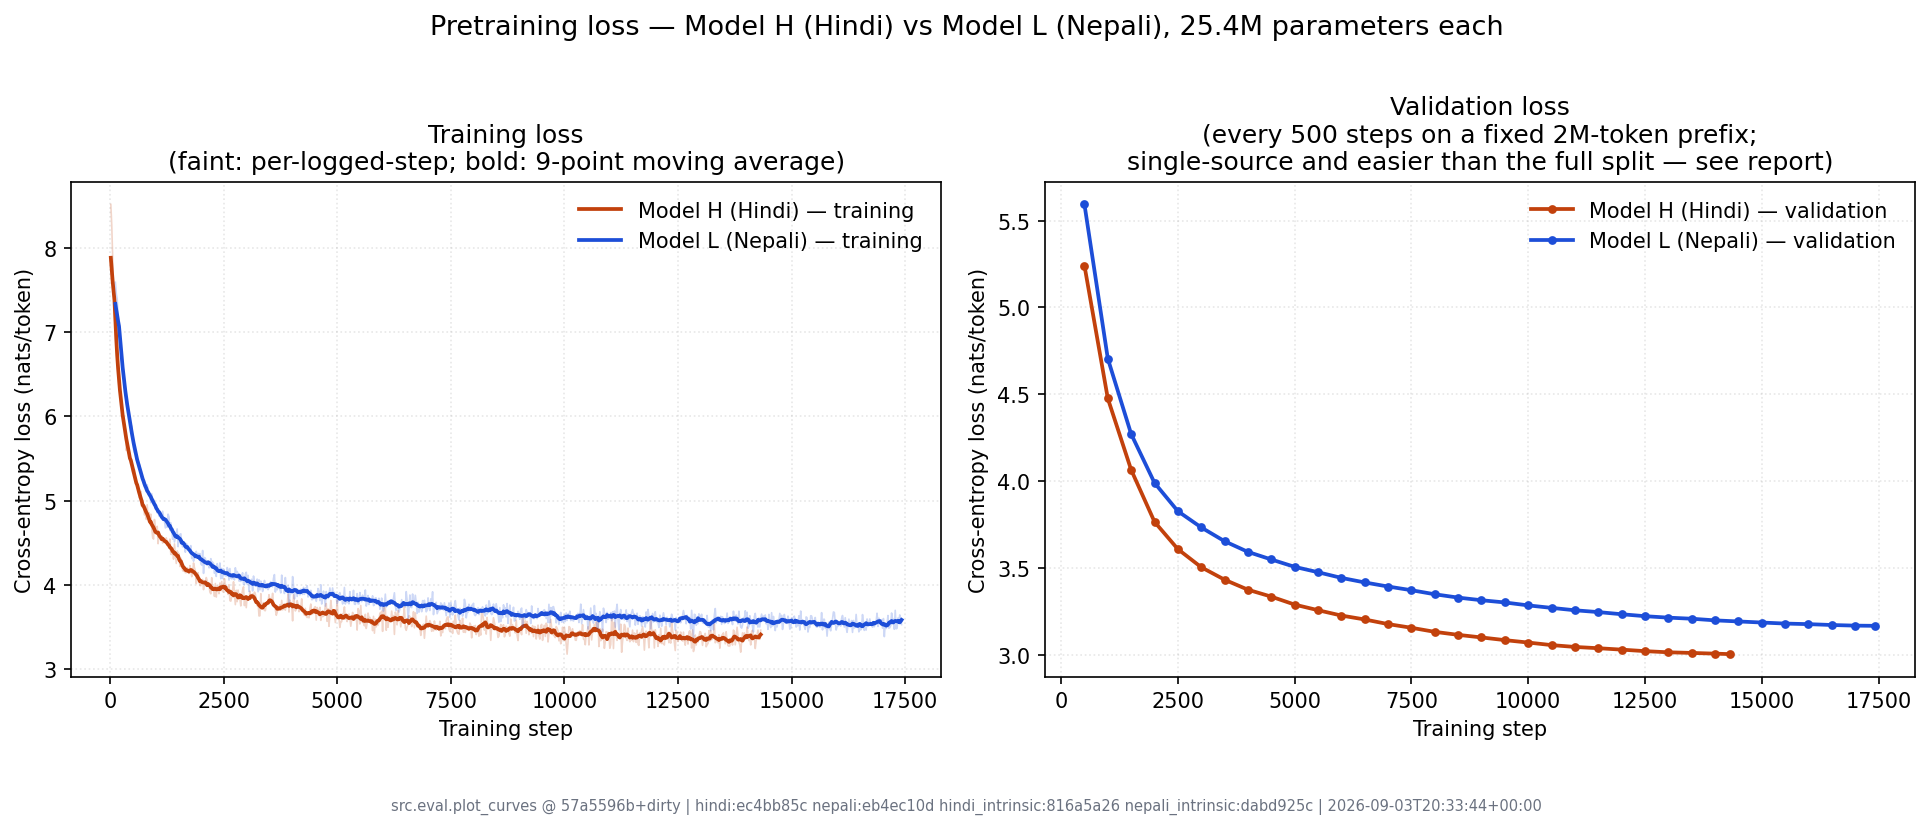
\includegraphics[width=\textwidth]{loss_curves}
  \caption{Training and validation loss for both models over one epoch.
  Validation loss falls monotonically in both runs and does not turn over,
  which is consistent with one epoch being close to compute optimal at this
  model size.}
  \label{fig:loss}
\end{figure*}

\begin{figure*}[tb]
  \centering
  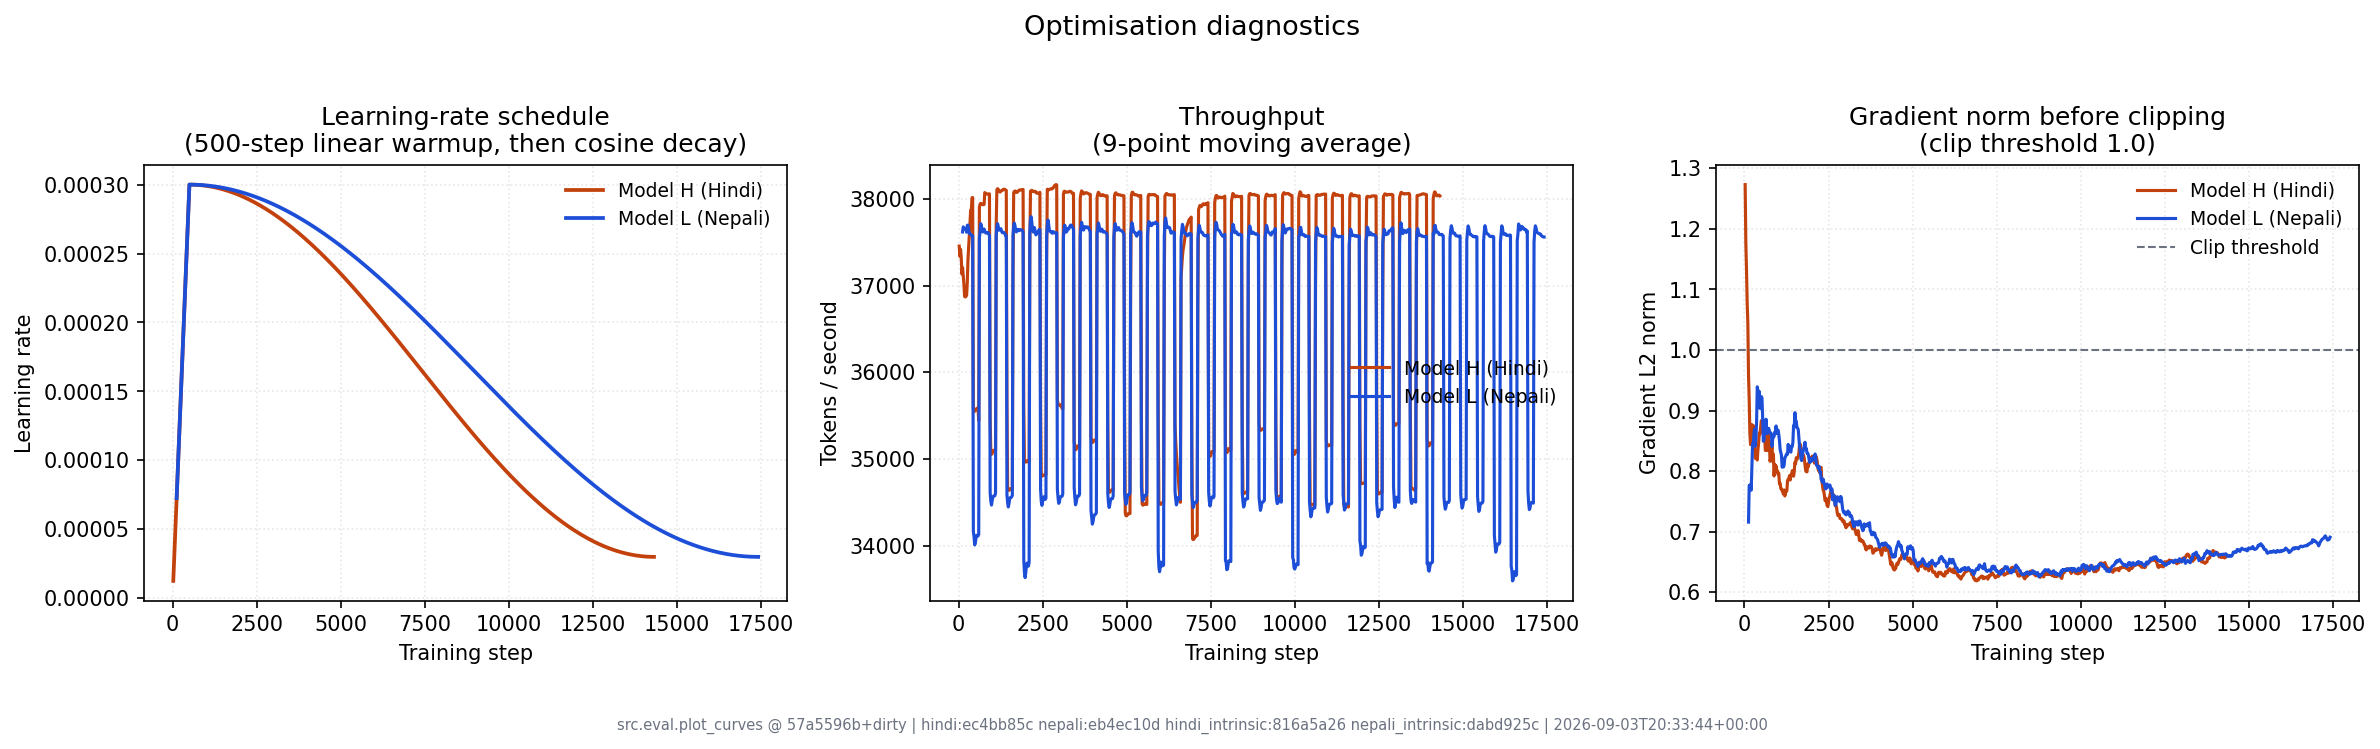
\includegraphics[width=\textwidth]{optimisation_diagnostics}
  \caption{Learning rate, gradient norm and throughput during pretraining.
  Gradient norms stay bounded after warmup and throughput is flat at roughly
  36,500 tokens per second in both runs, despite the different micro batch
  sizes.}
  \label{fig:optdiag}
\end{figure*}

I trained each model for one epoch.

The model had about 25.4 million parameters. Using around 20 tokens per parameter gives roughly 508 million tokens, which was close to the amount of training data I had.

The Hindi model was trained on 468,638,315 tokens and the Nepali model was trained on 571,113,472 tokens. This gave 18.5 tokens per parameter for Hindi and 22.5 for Nepali.

I used gradient accumulation so that both models processed 32,768 tokens per optimisation step.

The Hindi model used a micro batch of 16 with accumulation over 4 steps. The Nepali model used a micro batch of 32 with accumulation over 2 steps.

A large batch was not possible because the GPU memory was limited. The logits tensor itself becomes very large because the model has 8,000 possible output tokens.

The total pretraining time was about 12.5 GPU hours. The Hindi run took 3.69 hours and the Nepali run took 4.87 hours.

\subsection{Language Modelling Results}

\begin{figure}[tb]
  \centering
  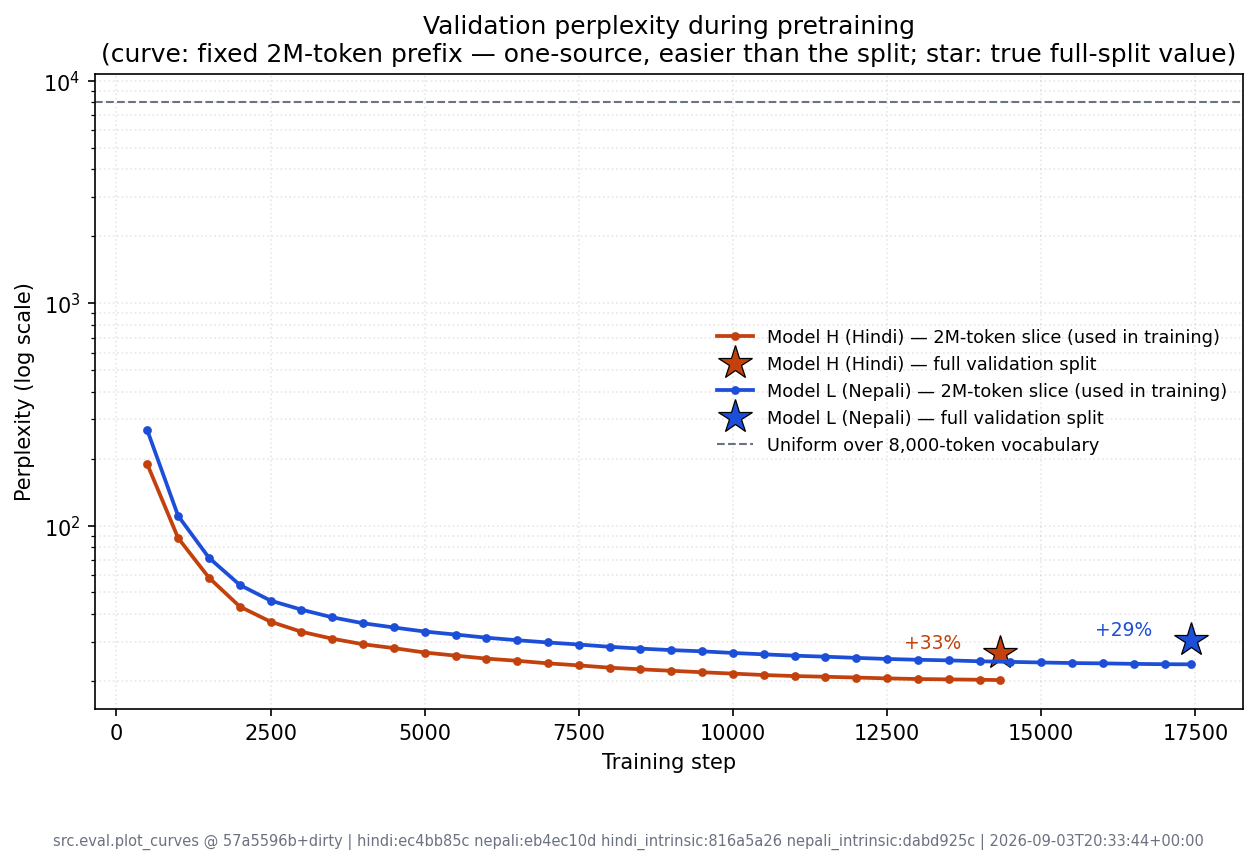
\includegraphics[width=\columnwidth]{val_perplexity}
  \caption{Validation perplexity during pretraining. Hindi stays below Nepali
  throughout. This is a per token measure, so it reflects tokenizer fertility
  as well as model quality.}
  \label{fig:valppl}
\end{figure}

The main results were:

\begin{table}[h]
\centering
\begin{tabular}{lrr}
\toprule
Metric & Hindi & Nepali \\
\midrule
Test cross entropy & 3.2885 & 3.4228 \\
Test perplexity & 26.80 & 30.65 \\
Bits per byte & 0.5371 & 0.4495 \\
Bits per character & 1.3636 & 1.1964 \\
Characters per token & 3.479 & 4.127 \\
\bottomrule
\end{tabular}
\end{table}

Based on cross entropy and perplexity, Hindi performed better. Hindi had a test perplexity of 26.80 while Nepali had 30.65.

But when I looked at bits per character, Nepali performed better. Nepali had 1.1964 bits per character compared to 1.3636 for Hindi.

At first this was confusing because both metrics seemed to be saying different things. The reason is the tokenizer. The two tokenizers do not represent the same amount of text in each token. Nepali had 4.127 characters per token while Hindi had 3.479.

So a Nepali token represents more text on average. Perplexity measures prediction at the token level, so the two values are not completely equivalent across languages.

This taught me that a metric should not be interpreted without looking at how it is calculated. For comparing two languages, bits per character gave me a more useful normalisation because both languages use the same script.

\subsection{Text Generation}
I also tested the models by generating text using different temperature values.

I found that greedy generation produced a lot of repetition. For example, the Hindi model had 80.9 percent repeated 4 grams in greedy generation, while the human reference had only 2.8 percent.

At temperature 1.0, the diversity statistics were much closer to the human reference.

BLEU was not very useful for this experiment. BLEU is more natural for tasks such as translation where there are expected reference outputs. In open ended generation, the model can generate a good sentence which is different from the one reference sentence. In that case BLEU can still give a very low score.

Therefore, I found the repetition and diversity measures more useful for understanding the generation behaviour.

\subsection{Attention Analysis}

\begin{figure*}[tb]
  \centering
  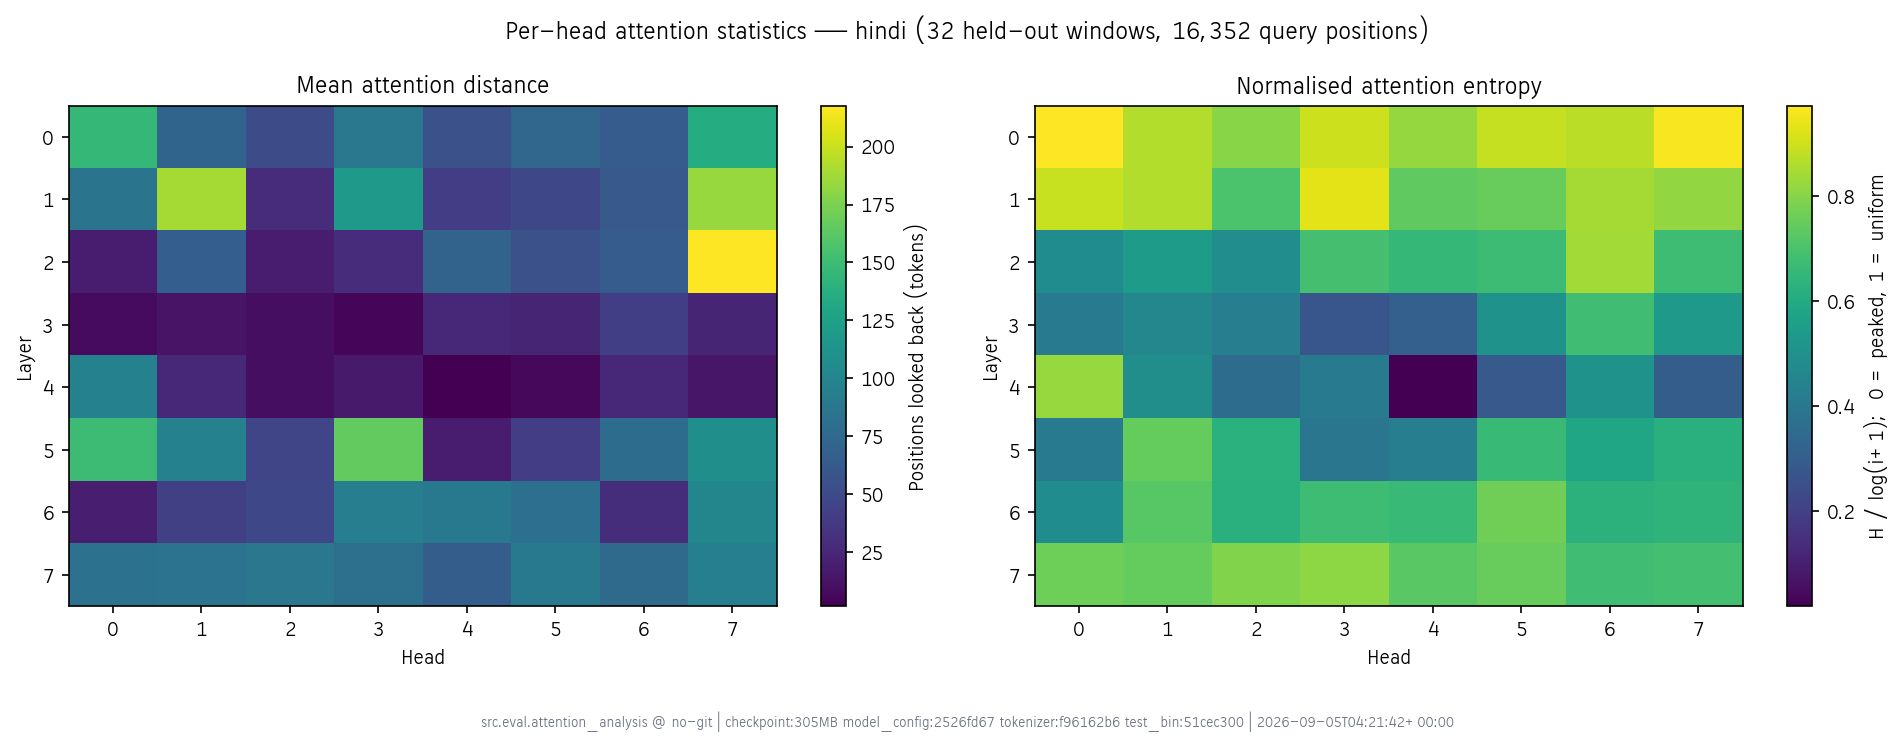
\includegraphics[width=0.49\textwidth]{hindi_attention_head_summary}\hfill
  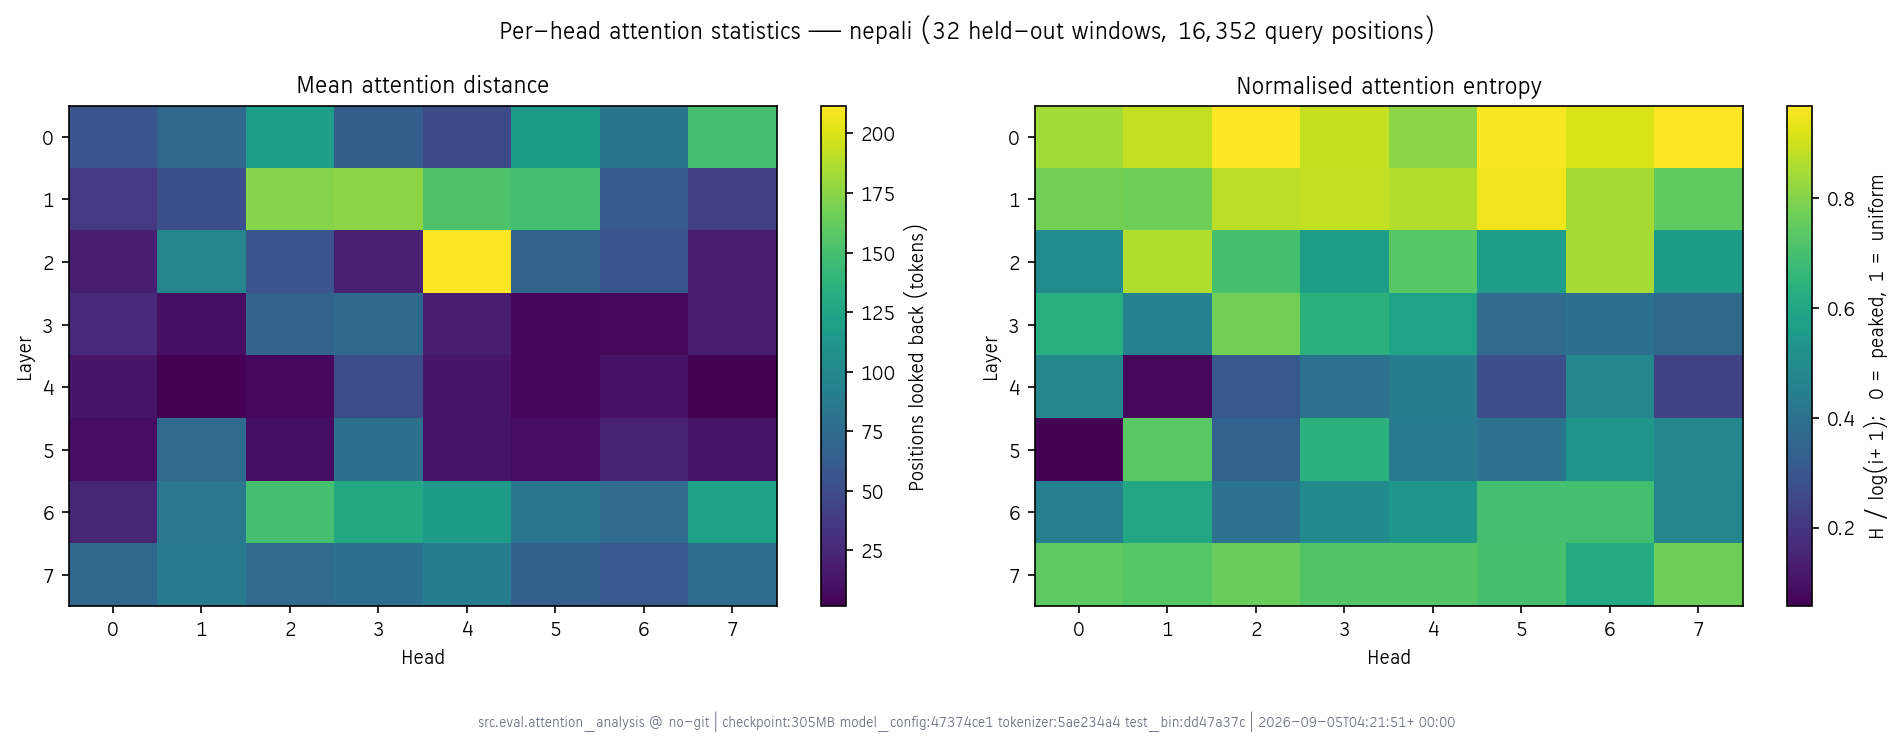
\includegraphics[width=0.49\textwidth]{nepali_attention_head_summary}
  \caption{Per head attention statistics for Hindi (left) and Nepali (right).
  The two models share no data, no vocabulary and no weights, yet every
  aggregate statistic agrees to within about four percent.}
  \label{fig:headsummary}
\end{figure*}

I also studied the attention patterns of the two pretrained models.

The average attention distance was 65.6 for Hindi and 63.3 for Nepali. The values were quite close.

This was interesting because the two models did not share their training data, tokenizer or weights. Still, their overall attention statistics were similar.

This suggests that some of the attention behaviour may be coming mainly from the Transformer architecture and the language modelling objective instead of the particular dataset.

The main attention pattern was also similar. Attention was more spread out in some layers and became more local in the middle layers before becoming broader again later.

\section{Phase 3: Reasoning Finetuning}

\subsection{Creating the Reasoning Dataset}
In Phase 3, I created a synthetic reasoning dataset for Hindi and Nepali.

There were 55,000 examples for each language and 10 reasoning families. The examples involved quantities, comparisons and relationships between different entities.

I generated the examples programmatically instead of using another language model. This was useful because I knew the correct answer for every generated example.

Some examples required the model to combine multiple statements. For example, if A is greater than B and B is greater than C, the model needs to use both statements to determine the relation between A and C.

I also used separate entity pools for training and testing. This was done so that the model could not simply memorise which answer belongs to a particular name.

There were also separate checks for data leakage. The cross split checks all returned zero. This gave me more confidence that the test results were actually testing unseen examples.

\subsection{Devanagari Numbers}
I used Devanagari numerals in the synthetic dataset instead of ASCII numbers.

This produced an interesting tokenizer result. The Hindi vocabulary contained 42 Devanagari numeral pieces while the Nepali vocabulary contained 158.

The number of tokens used for each stated quantity was 2.044 for Hindi and 1.458 for Nepali.

This means the Nepali tokenizer was better at representing the numbers used in the synthetic dataset. This probably happened because Nepali web text contains many Bikram Sambat dates.

However, the Nepali tokenizer also lost more of its fertility advantage when used on the synthetic data. So the same property of the corpus helped it with numerals but also made it less robust outside its original data.

\subsection{Three Test Sets}
I did not use only one accuracy score. I created different test conditions to understand why the model succeeds or fails.

One test used entities that had already appeared during training. Another used unseen entities with familiar phrasing. The final test used unseen entities and held out phrasing.

This was important because a single accuracy number can hide the reason for a failure.

For example, a model can get a low score because it cannot understand the task, or because it knows the task but has memorised the training names. These are very different problems.

\subsection{Few Shot Evaluation}

\begin{figure*}[tb]
  \centering
  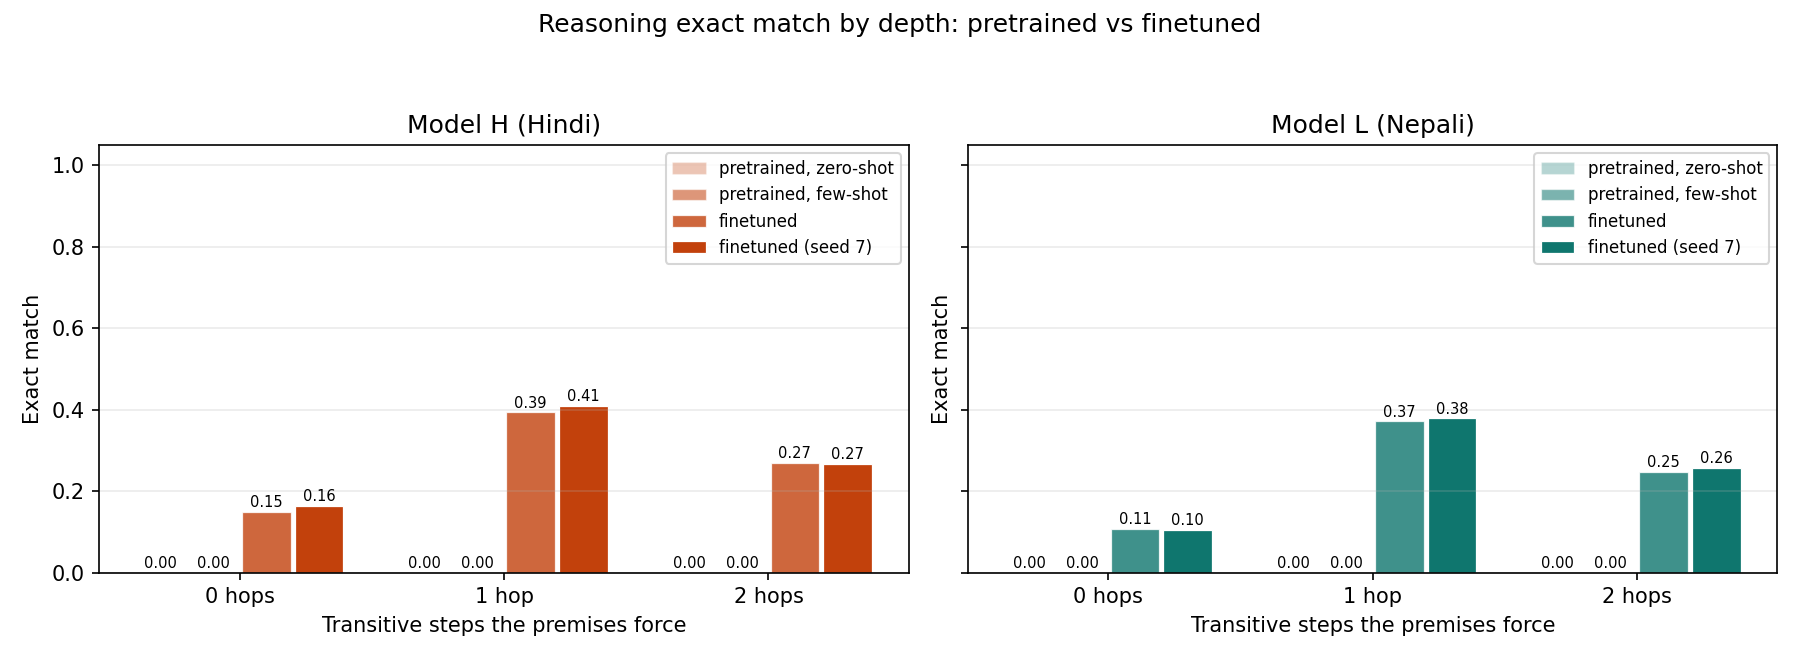
\includegraphics[width=\textwidth]{reasoning_accuracy}
  \caption{Exact match by reasoning depth for both models. Zero shot and few
  shot both score zero at every depth, so only the finetuned models appear
  above the axis.}
  \label{fig:reasonacc}
\end{figure*}

Before finetuning, both models had zero exact match accuracy on the unseen entity test.

I then gave four examples before the question. This made a large difference to the output format.

For the Hindi model, the format rate became 99.98 percent. However, the exact match accuracy was still 0 percent.

This was a very useful result for me. It showed that the model could learn how the answer should look without actually learning how to solve the reasoning task.

So just because a model gives the correct format does not mean that it understands the problem.

\section{Memorisation of Entity Names}
After finetuning, I looked at performance based on the type of answer required.

The results showed a clear difference between relation word answers and entity name answers.

For the aggressive finetuning recipe, Hindi had an accuracy of 0.5335 on relation word answers but only 0.0540 on entity name answers. Nepali had 0.5360 on relation word answers and 0.0000 on entity name answers.

This was a very important finding.

I looked at some of the wrong generated answers. The model often produced names which had appeared in the training set even when the correct answer was a completely new name.

For example, if the correct answer was one unseen person, the model might output another person from the training data.

This suggests that the model learned a shortcut. When the question asked for an entity, it often selected one of the names it had already seen instead of actually calculating the answer.

The seen entity control test supports this idea. Hindi achieved 0.6226 accuracy when the test used entities from the training pool. The accuracy became much lower when the entities were unseen.

Therefore, I concluded that the main problem was not simply the question wording. The model had learned to associate the task with the names present in the training data.

\section{Finetuning Caused Forgetting}

\begin{figure*}[tb]
  \centering
  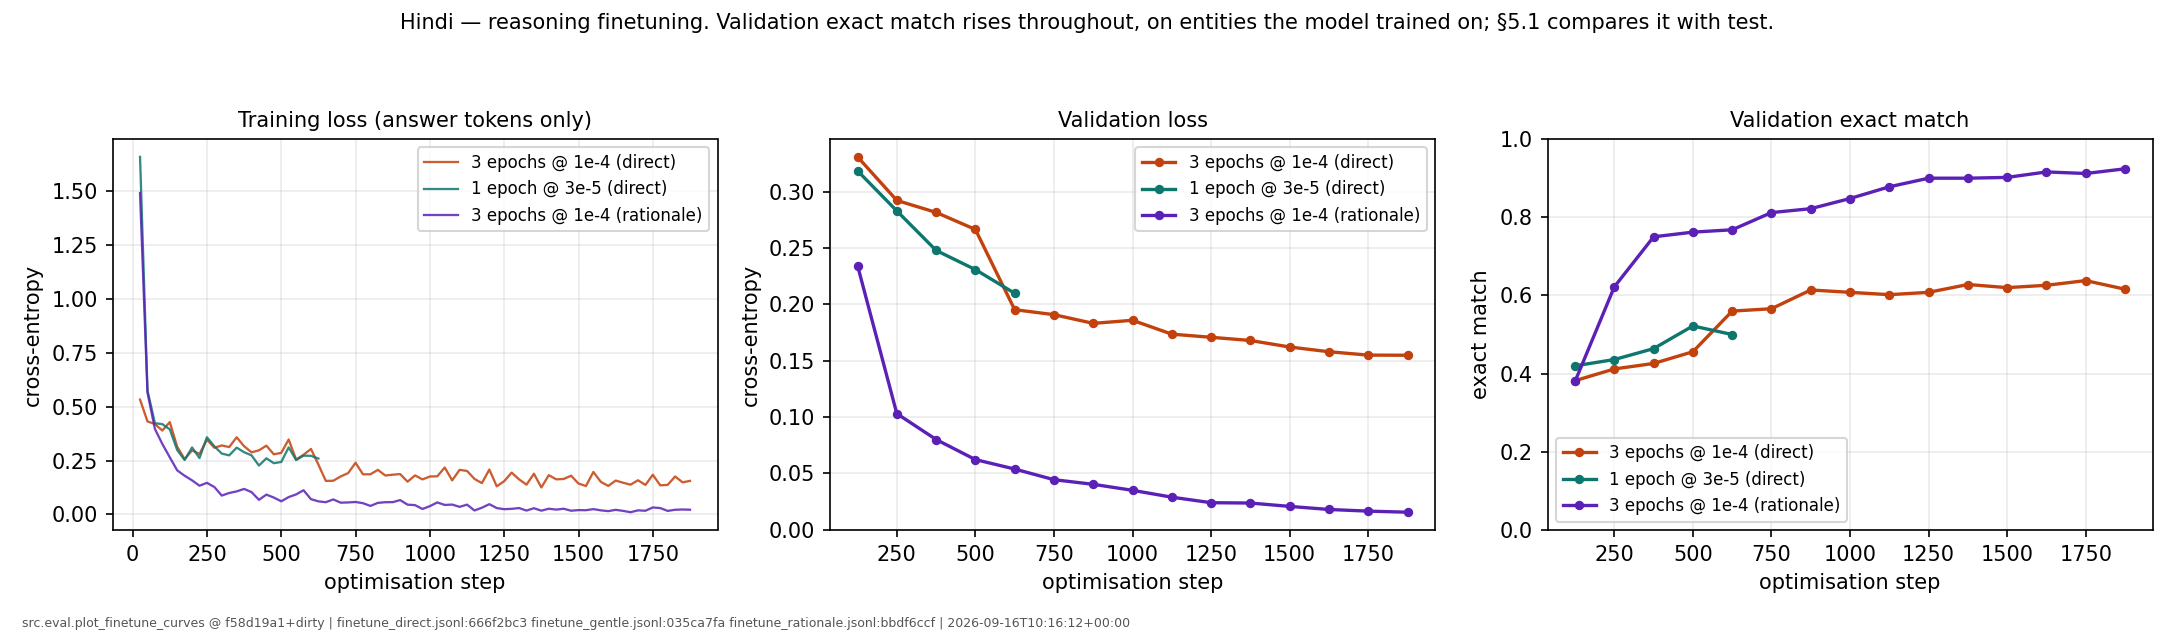
\includegraphics[width=\textwidth]{finetune_curves_hindi}
  \caption{Hindi finetuning. The rationale run reaches the lowest validation
  loss and the highest validation exact match of the three runs, and still
  scores lowest on the held out test set. The validation split draws its
  entities from the training pool, so it cannot detect memorisation of entity
  names.}
  \label{fig:ftcurveshi}
\end{figure*}

\begin{figure*}[tb]
  \centering
  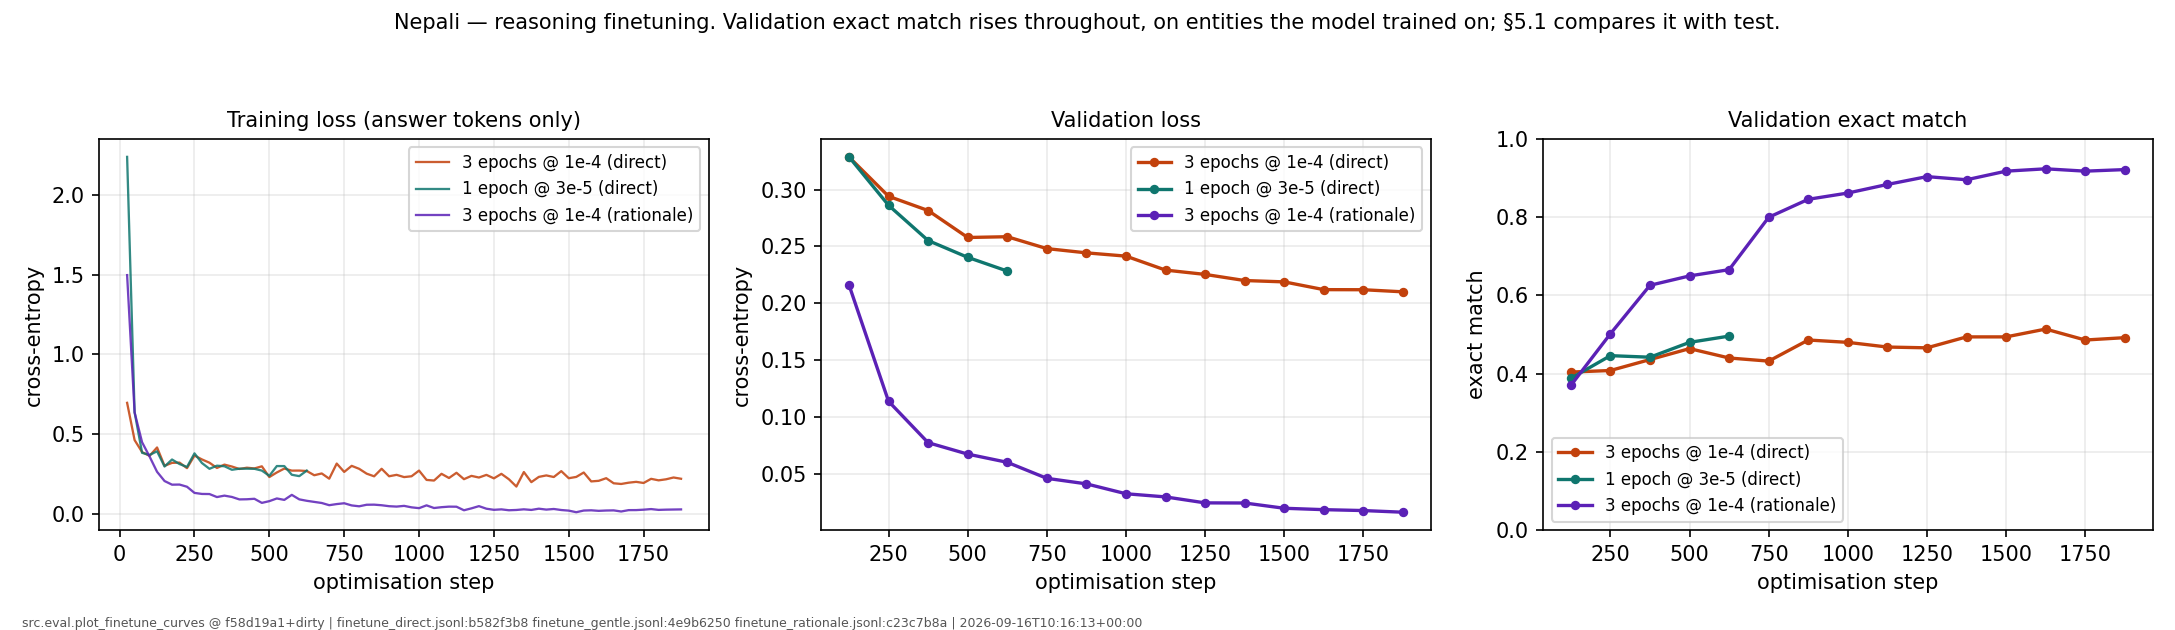
\includegraphics[width=\textwidth]{finetune_curves_nepali}
  \caption{Nepali finetuning. The same pattern appears. Validation loss and
  validation exact match both improve throughout and give no indication of the
  test set result.}
  \label{fig:ftcurvesne}
\end{figure*}

I first used an aggressive finetuning recipe with 3 epochs and a learning rate of 0.0001.

The language modelling ability became much worse after this.

The Hindi validation perplexity increased from 20.19 before finetuning to 1115.21 after finetuning. For Nepali, it increased from 23.77 to 2801.61.

This was a very large change.

I originally expected finetuning to be a relatively small change because the number of finetuning steps was much smaller than the number of pretraining steps. But this assumption was wrong.

I then tried a gentler recipe with only 1 epoch and a learning rate of 0.00003.

The results were much better. Hindi had a perplexity of 25.00 and Nepali had a perplexity of 29.40 after finetuning.

The language modelling ability retained was around 96 percent for both models, compared with only 33 percent for Hindi and 18 percent for Nepali with the aggressive recipe.

The gentle recipe also improved exact match accuracy. Hindi increased from 0.2458 to 0.2992 and Nepali increased from 0.2144 to 0.2320.

This showed me that the aggressive recipe was simply too strong for this task.

\section{Attention After Finetuning}

\begin{figure*}[tb]
  \centering
  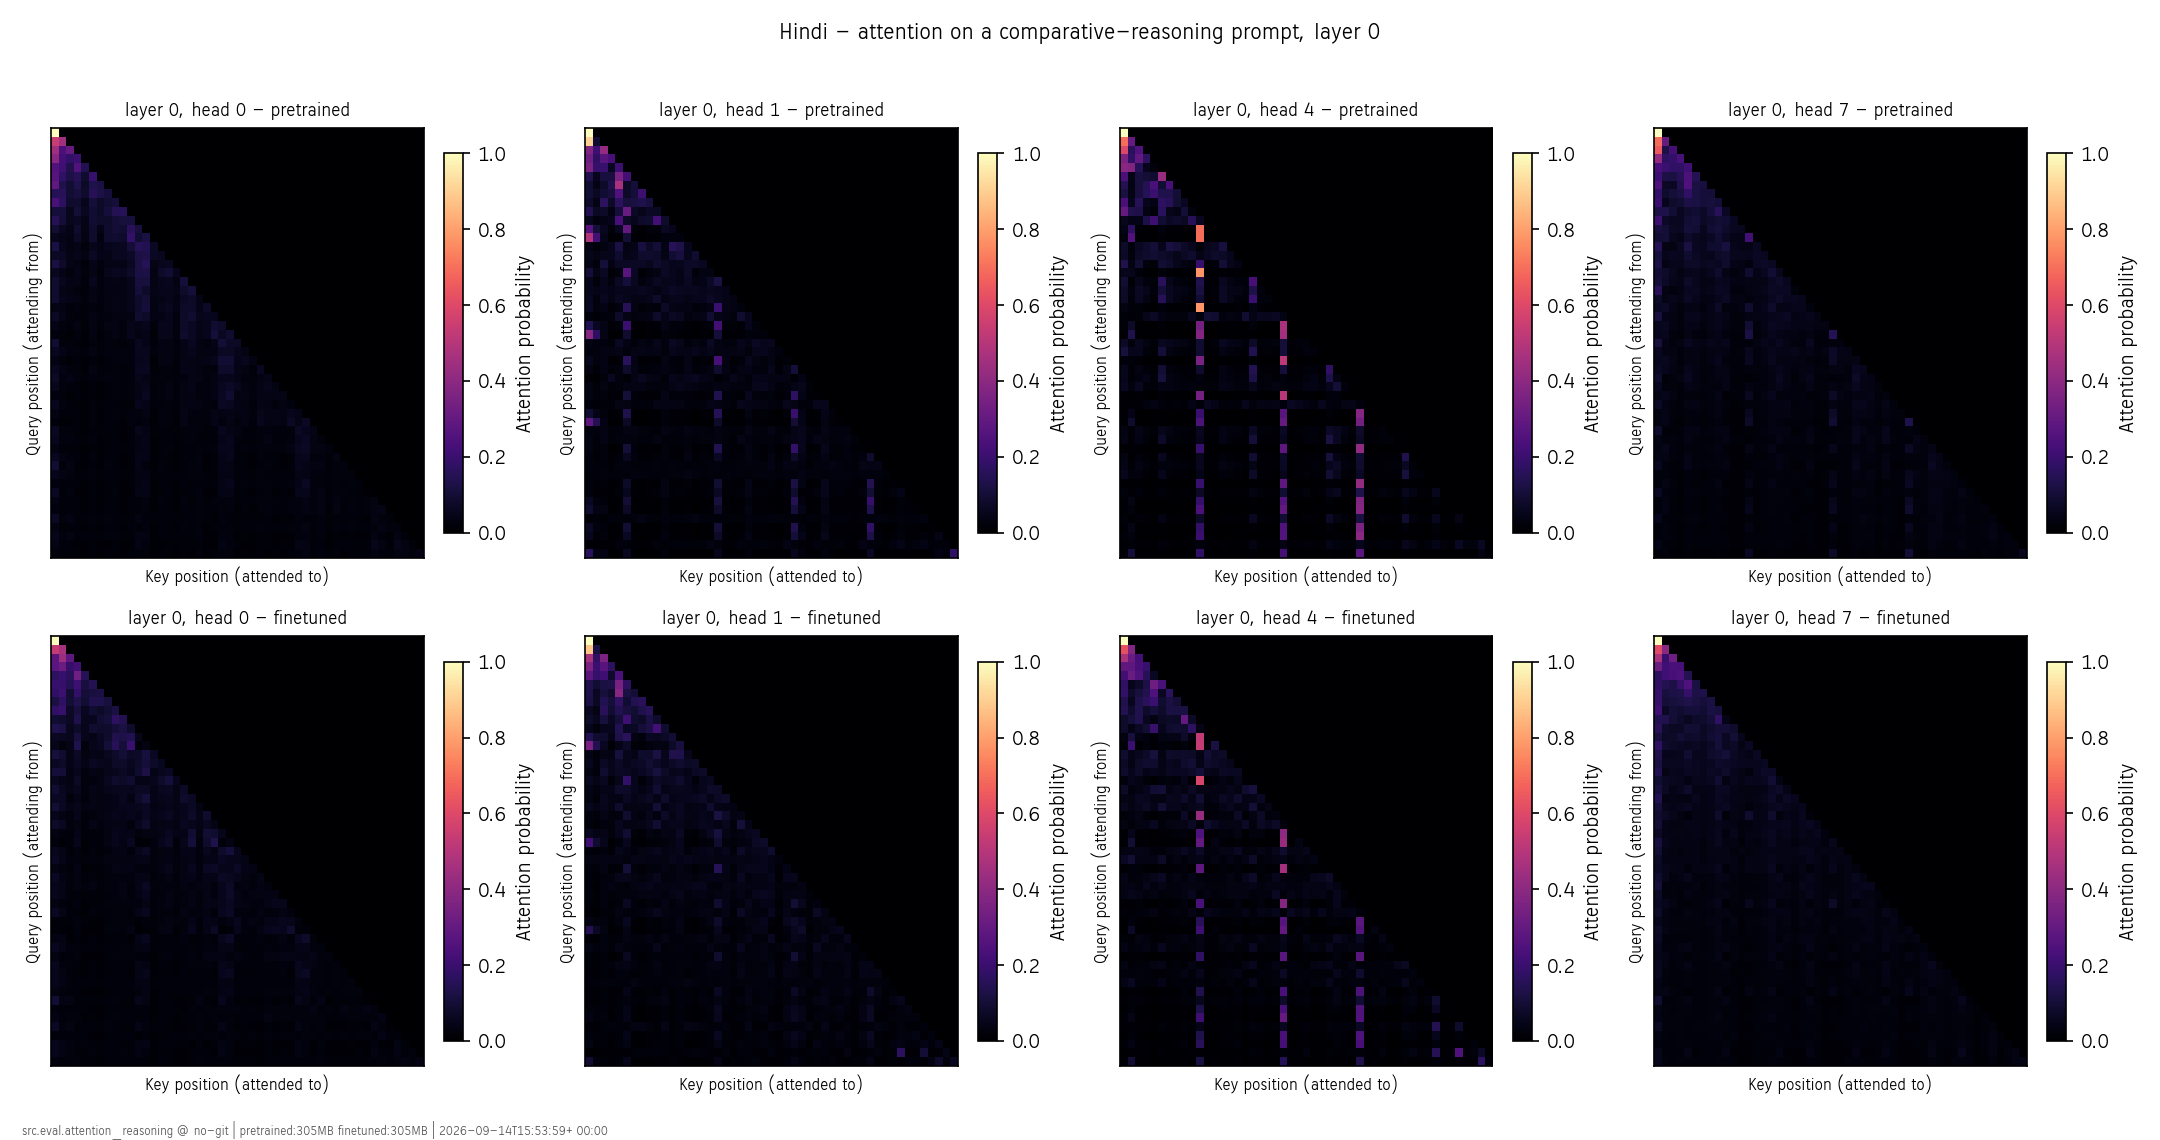
\includegraphics[width=\textwidth]{hindi_reasoning_attention_direct_layer0}
  \caption{Hindi, layer 0, which is an early layer. The pretrained checkpoint
  is on the top row and the finetuned checkpoint is beneath it, showing four
  heads of the same layer on the same comparative reasoning prompt.}
  \label{fig:attnhi0}
\end{figure*}

\begin{figure*}[tb]
  \centering
  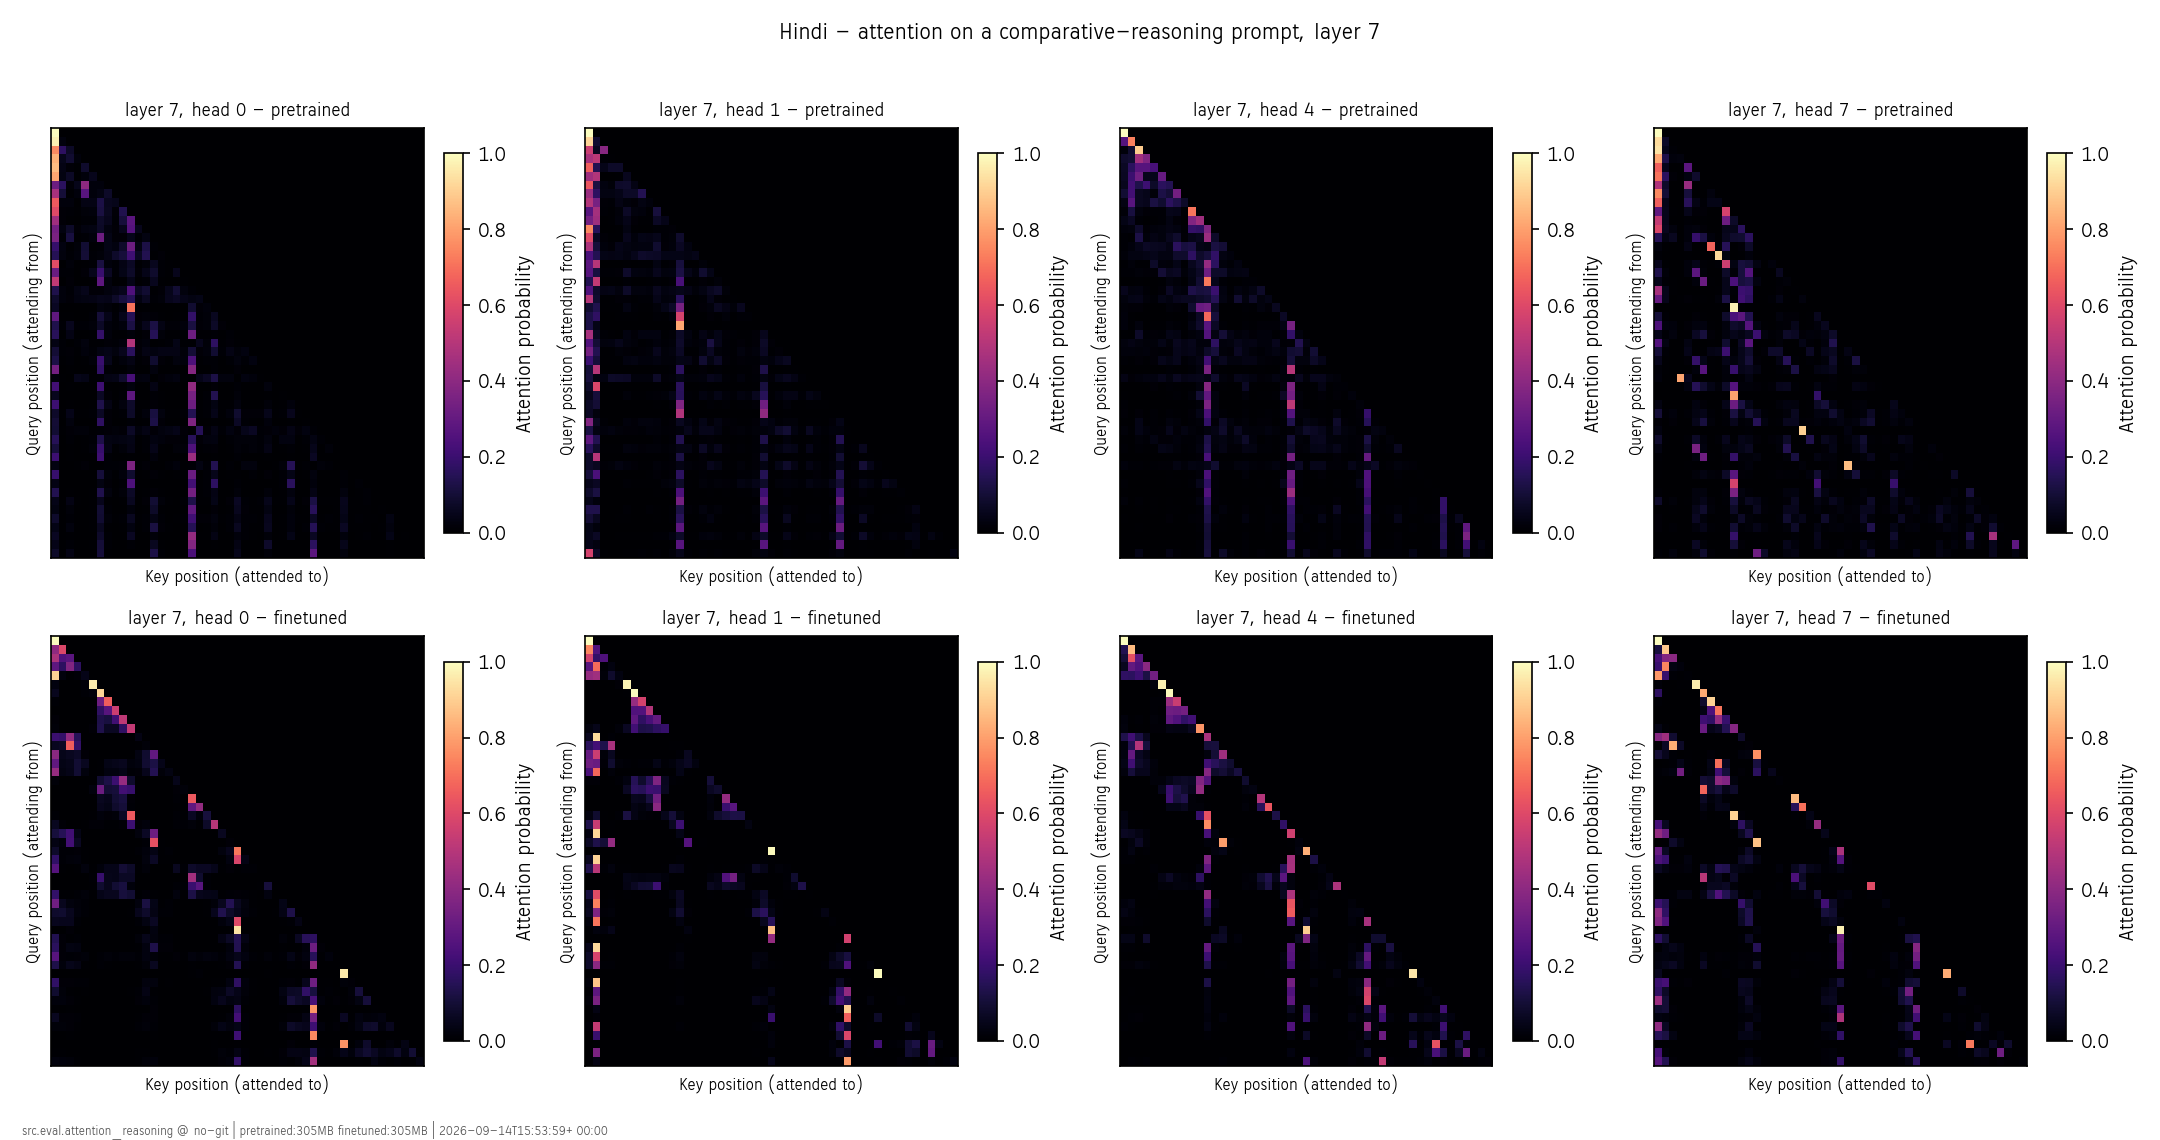
\includegraphics[width=\textwidth]{hindi_reasoning_attention_direct_layer7}
  \caption{Hindi, layer 7, which is a late layer. Mean attention distance
  decreased in all eight layers after finetuning, and the most common change in
  head role was from content based attention to local attention.}
  \label{fig:attnhi7}
\end{figure*}

\begin{figure*}[tb]
  \centering
  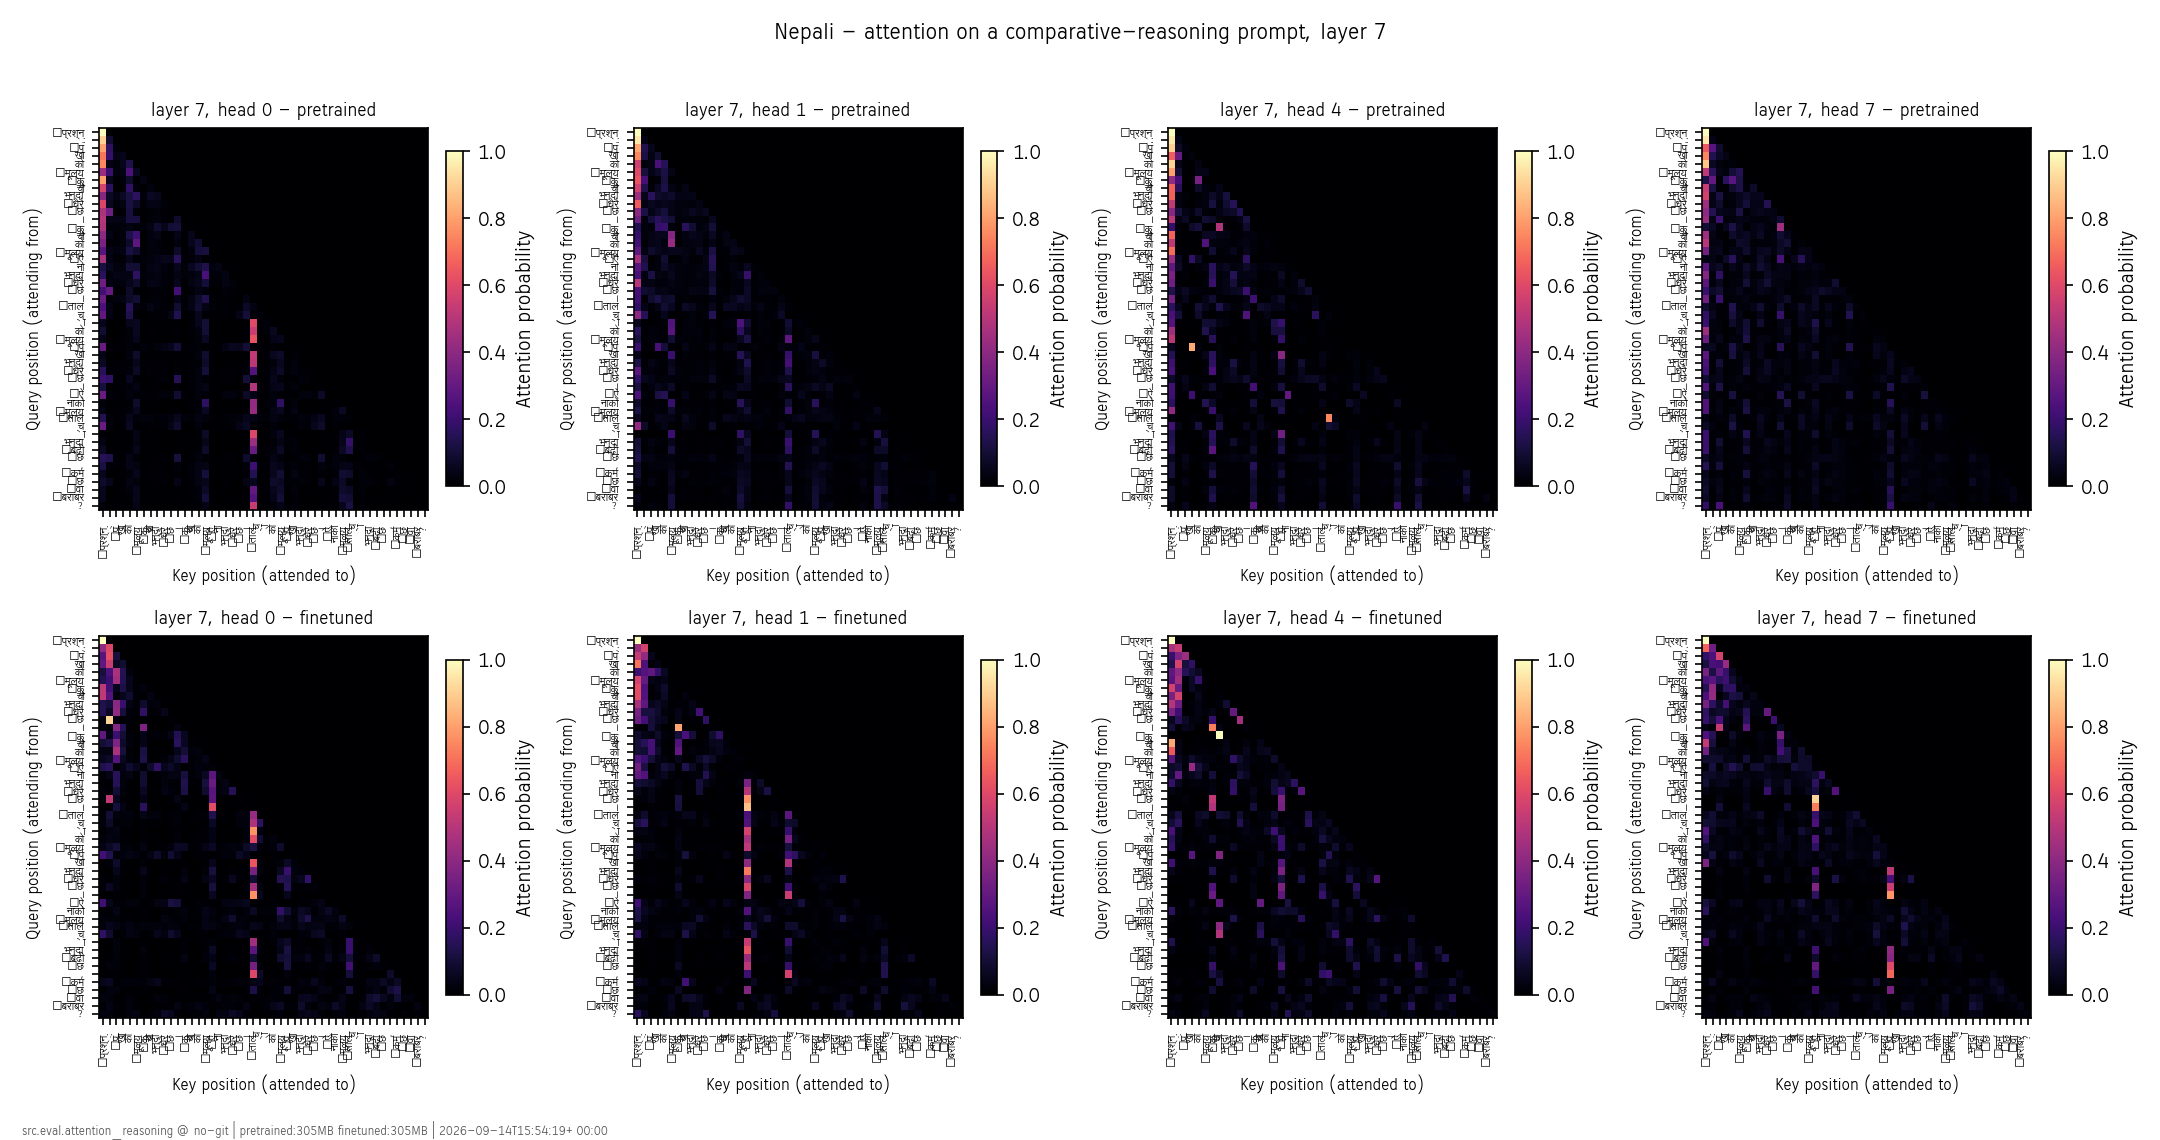
\includegraphics[width=\textwidth]{nepali_reasoning_attention_direct_layer7}
  \caption{Nepali, layer 7, which is a late layer. Both models end at the same
  mean attention distance of 7.70 after finetuning, having started 0.56 apart.}
  \label{fig:attnne7}
\end{figure*}

I also compared attention before and after finetuning.

For Hindi, the mean attention distance changed from 8.76 to 7.70. For Nepali, it changed from 8.20 to 7.70.

All 8 layers showed a decrease in attention distance in both models.

I also found that 21 out of 64 Hindi attention heads and 20 out of 64 Nepali heads changed their roles.

The main change was from content based attention towards more local attention.

This matches another result from the reasoning experiment. The models had very high format rates, around 0.96 to 1.00, but exact match accuracy was only around 0.21 to 0.25.

So the models became better at following the local structure and format of the synthetic task, but this did not mean that they became good at reasoning.

\section{Bonus Experiment: Removing Positional Embeddings}

\begin{figure*}[tb]
  \centering
  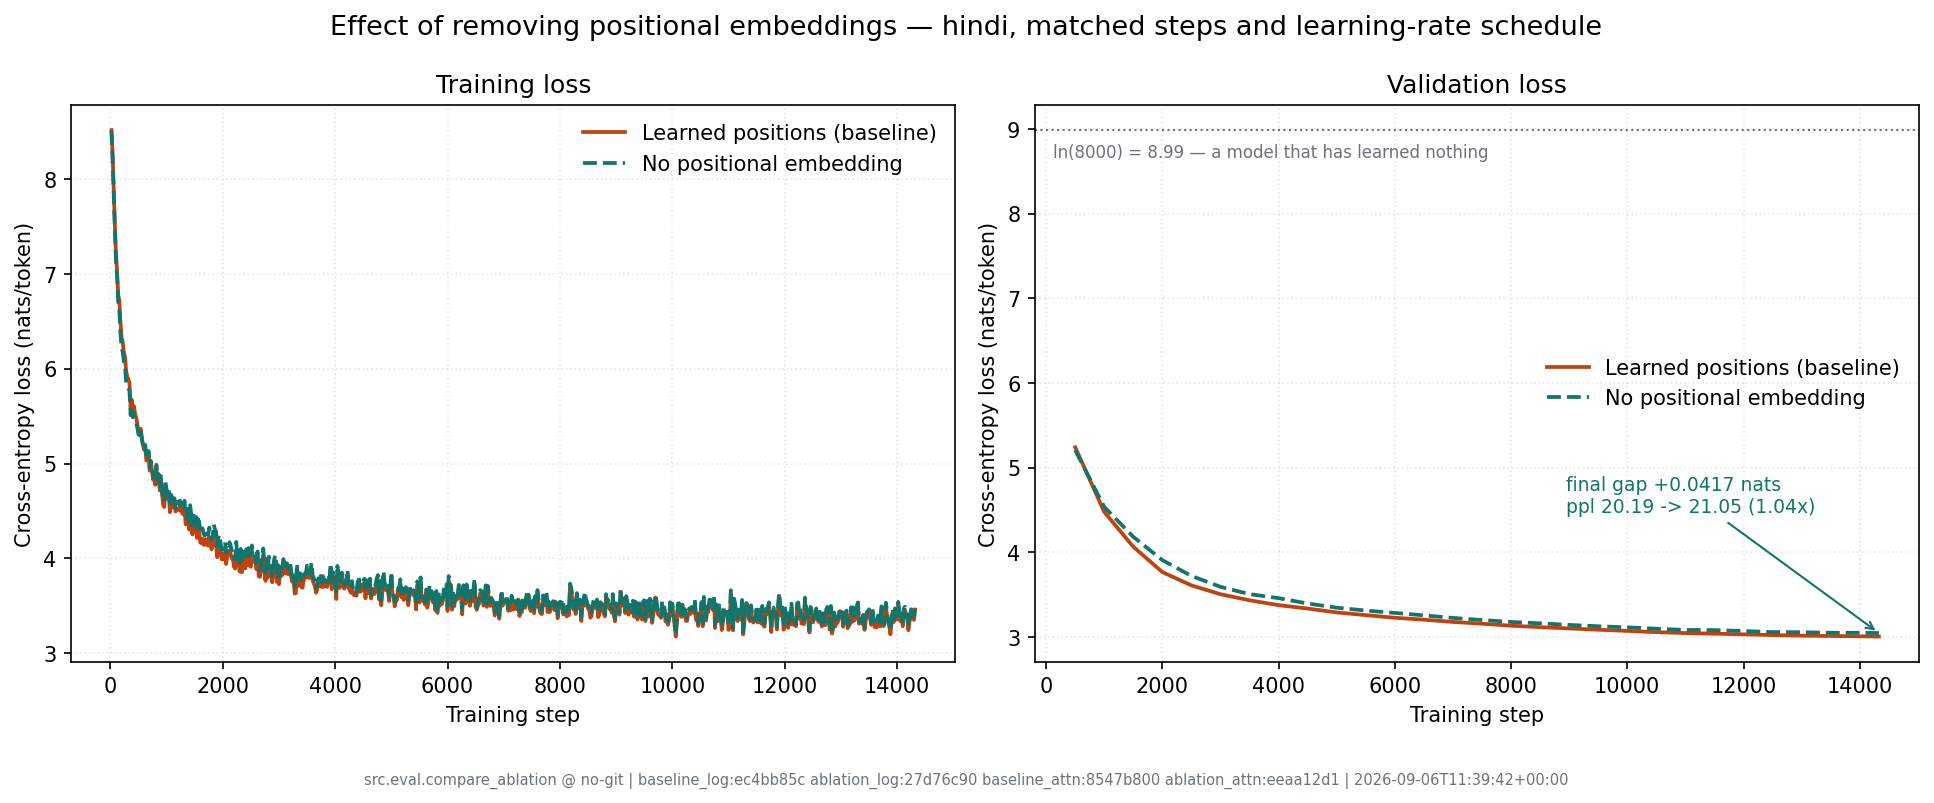
\includegraphics[width=\textwidth]{hindi_ablation_nopos_loss}
  \caption{Hindi with and without learned positional embeddings, matched on
  seed, steps, batch composition and learning rate schedule. The two curves are
  almost superimposed, which is the 3.4 percent perplexity difference seen as a
  training curve.}
  \label{fig:nopos}
\end{figure*}

For the bonus experiment, I retrained the Hindi model without learned positional embeddings.

The original model had a perplexity of 26.80. The model without positional embeddings had a perplexity of 27.70.

This was an increase of only 3.4 percent.

I expected removing positional information to have a bigger effect. But the causal mask itself gives some information about position. A token at a later position can see more previous tokens than a token at an earlier position.

So even without learned positional embeddings, the model still has some information about where it is in the sequence.

The cross entropy increased from 3.2885 to 3.3216.

This experiment also taught me that a proper ablation needs to keep the other training conditions the same. In particular, the learning rate schedule had to be matched. Otherwise, the difference could come from training rather than from removing positional embeddings.

\section{Reflections}
There were several decisions in the project where the actual results were different from what I expected.

The first was the tokenizer decision. Based only on fertility, Unigram was slightly better. I still selected BPE for other reasons. Looking back, I think I should have tested both tokenizers by actually pretraining the same model with both of them. That would have given a much stronger basis for the decision.

The second was finetuning. I thought that 1,875 finetuning steps would be a small change compared with the much larger number of pretraining steps. Instead, the aggressive recipe destroyed most of the language modelling ability. I learned that the number of steps alone does not tell me how much the weights will change.

The third problem was the validation entity pool. I used entities from the training pool in validation. Because of this, the validation results could not properly detect memorisation of entity names. The validation score looked good even though the model failed on unseen names.

A better design would have used a completely separate entity pool for validation.

Another prediction that was wrong was about reasoning depth. I expected accuracy to decrease when the number of reasoning steps increased. Instead, the one step examples sometimes performed better than the zero step examples. Later I found that reasoning depth was mixed with answer type. Many of the zero step examples asked for entity names, which were much harder for the model.

I also had a prediction about numeral tokenization. I expected the Nepali tokenizer to give better reasoning performance on quantity based questions because it had more numeral pieces. This result changed when I used the gentler finetuning recipe. Because the direction changed, I cannot confidently say that the tokenizer caused the difference.

These results made me understand why experimental design is so important. If multiple things change at the same time, it becomes difficult to know what actually caused the result.

\section{Limitations}
There are several limitations in my project.

First, I only trained a small number of models. Because of this, the results should not be treated as a general conclusion about all Hindi and Nepali language models.

Second, the two datasets differ in several ways. Corpus size, source distribution, fertility and domain distribution are all different. Therefore, I cannot say that one particular factor caused the difference between the models.

Third, the reasoning task is quite narrow. It mainly tests comparative ordering using synthetic sentences. Good performance on this task would not mean that a model can perform general reasoning.

Fourth, the reasoning dataset is synthetic and based on templates. Real world reasoning is much more complicated.

Fifth, the model size is only about 25 million parameters. This is very small compared with modern large language models. Therefore, poor performance on the reasoning task should not be treated as a conclusion about the reasoning ability of the languages themselves.

Finally, attention analysis can show where the model is looking, but it cannot directly tell me why the model is looking there. So I should not treat the attention results as a complete explanation of the model behaviour.

\section{Conclusion}
In this project, I built two language models for Hindi and Nepali. I kept their architecture, vocabulary size and parameter count the same so that I could study the effect of the training data more clearly.

During Phase 1, I learned that data cleaning is a very important part of language model training. The duplicate detection experiment was especially useful because I found 1,718 identical Nepali article texts even though the URLs were different. This showed why checking only URLs is not enough.

During Phase 2, I found that different evaluation metrics can give different results. Hindi had better perplexity, but Nepali had better bits per character. This difference was related to how the tokenizers represented the text.

During Phase 3, I found that the models were much better at learning the expected answer format than actually solving the reasoning problem. The models also showed strong memorisation of entity names. When I tested unseen entities, their performance became very low.

The finetuning experiment was another major result. The aggressive recipe caused a huge amount of forgetting. The gentler recipe using one epoch and a lower learning rate gave better reasoning accuracy while retaining around 96 percent of the original language modelling ability.

The biggest lesson I got from this project is that a model score by itself does not tell the whole story. I need to understand what the metric measures, how the dataset was made and whether there are hidden factors affecting the result.

Some of my predictions were wrong, but I think these failures were actually useful. They helped me understand the model better and also showed me how experimental design can affect the conclusions. Overall, this project gave me a better understanding of how data, tokenization, model architecture and finetuning interact with each other.

\end{document}
